\section{Problem 1: Quantum Harmonic Oscillator}

\

\subsection{Analytical methodology}

\subsubsection{Time-Independent Schrödinger Equation}

The time-independent Schrödinger Equation is
\begin{align*}
    H\ket{\psi} &= E \ket{\psi} 
\end{align*}
%
where the Hamiltonian $H$ is
\begin{align*}
    H &= T + V
\end{align*}
%
$T$ and $V$ are the kinetic and potential operators, respectively.

\subsubsection{Quantum Harmonic Oscillator Hamiltonian}

The Hamiltonian of the quantum harmonic oscillator is
\begin{align*}
    H &= \frac{p^2}{2m} + \frac{1}{2} m \omega^2 x^2
\end{align*}
%
where $p$ and $x$ are the momentum and position operators, respectively.

\subsubsection{Projection onto 1D Position Space}

When projected onto one dimension of position space, the time-independent Schrödinger equation becomes
\begin{align*}
    H\psi(x) &= E \psi(x) \\
    -\frac{\hbar^2}{2m}\frac{\partial^2 \psi(x)}{\partial x^2} + V(x)\psi(x) &= E \psi(x)
\end{align*}

\subsubsection{Resulting Differential Equation}

The time-independent Schrödinger equation is a differential equation:
\begin{align*}
    \frac{\partial^2 \psi(x)}{\partial x^2} + \frac{2m(E-V(x))}{\hbar^2}\psi(x) &= 0
\end{align*}

\subsubsection{Analytical Energy Spectrum}

The eigenvalues of $H$ form a spectrum of values called the \textit{energy spectrum} of the system described by $H$. For the quantum harmonic oscillator, the energy spectrum is \cite[page 51]{Griffiths2018}:
\begin{align*}
    E_n &= \hbar\omega\Big(n+\frac{1}{2}\Big), \quad n=0,1,2,\dots
\end{align*}

\subsubsection{Analytical Energy Spectrum}

The eigenwavefunctions of the quantum harmonic oscillator turn out to be Hermite polynomials and are given normalized by Griffiths and Schroeter \cite[page 52]{Griffiths2018} as
\begin{align*}
    \psi_n(x) &= \Big(\frac{m\omega}{\pi\hbar}\Big)^{1/4} \frac{1}{\sqrt{2^n n!}} H_n(\xi) e^{-\xi^2/2}, \quad \text{where } \xi = \sqrt{\frac{m\omega}{\hbar}}x
\end{align*}
%
and the first few $H_n$ are:
\begin{align*}
    H_0 &= 1 \\
    H_1 &= 2\xi \\
    H_2 &= 4\xi^2 - 2 \\
    H_3 &= 8\xi^3 - 12\xi \\
    H_4 &= 16\xi^4 - 48\xi^2 + 12 \\
    H_5 &= 32\xi^5 - 160\xi^3 + 120\xi
\end{align*}
















\subsection{Numerical methodology}

\subsubsection{Finite Computational Interval, Grid Definition, and Grid Spacing}

A position grid of $N$ points is constructed as follows
\begin{align*}
    x_i &= x_\text{min} + i\Delta x, \quad i=0,1,2,\dots,N-1
\end{align*}
%
where the grid spacing $\Delta x$ is
\begin{align*}
    \Delta x &= \frac{x_\text{max} - x_\text{min}}{N-1}
\end{align*}

\subsubsection{Finite Difference Approximation to the 2\textsuperscript{nd} Derivative in the Differential Equation}

Let $\psi(x)$ be defined on a continuous interval of $x$ and have continuous 1\textsuperscript{st} and 2\textsuperscript{nd} derivatives. The 2\textsuperscript{nd} derivative, $\partial^2 \psi(x)/\partial x^2$, at any interior point $a$ of the interval may be approximated as
\begin{align*}
    \Bigg(\frac{\partial^2 \psi(x)}{\partial x^2}\Bigg)_{x=a} &\approx \frac{\psi(a+\Delta x) + \psi(x-\Delta x) - 2\psi(a)}{(\Delta x)^2}
\end{align*}
%
On our discrete grid, $\psi(x)$ becomes discrete $\psi(x_i)$ where $i=0,1,2,\dots,N-1$ and its 2\textsuperscript{nd} derivative becomes
\begin{align*}
    \Bigg(\frac{\partial^2 \psi(x)}{\partial x^2}\Bigg)_{x=x_i} &\approx \frac{\psi(x_{i+1}) + \psi(x_{i-1}) - 2\psi(x_{i})}{(\Delta x)^2}
\end{align*}
%
that is, it is calculated from the wavefunction values at $x_{i-1},x$ and $x_{i+1}$.

\subsubsection{Construction of the Kinetic Energy Matrix}

Thus the kinetic energy operator at each point $x_i$ is
\begin{align*}
    -\frac{\hbar^2}{2m}\Bigg(\frac{\partial^2 \psi(x)}{\partial x^2}\Bigg)_{x=x_i} &\approx -\frac{\hbar^2}{2m}\frac{\psi(x_{i+1}) + \psi(x_{i-1}) - 2\psi(x_{i})}{(\Delta x)^2}
\end{align*}
%
Noting that the 2\textsuperscript{nd} derivative is defined only at interior points $x_1,\dots,x_{N-2}$ and taking $\psi(x_0) = \psi(x_\text{min}) = 0$ and $\psi(x_{N-1}) = \psi(x_\text{max}) = 0$, we get the kinetic energy operator at each interior point:
\begin{align*}
    -\frac{\hbar^2}{2m}\Bigg(\frac{\partial^2 \psi(x)}{\partial x^2}\Bigg)_{x=x_1} &\approx -\frac{\hbar^2}{2m}\frac{\psi(x_2) - 2\psi(x_1)}{(\Delta x)^2} \\
    -\frac{\hbar^2}{2m}\Bigg(\frac{\partial^2 \psi(x)}{\partial x^2}\Bigg)_{x=x_2} &\approx -\frac{\hbar^2}{2m}\frac{\psi(x_{3}) + \psi(x_1) - 2\psi(x_2)}{(\Delta x)^2} \\
    -\frac{\hbar^2}{2m}\Bigg(\frac{\partial^2 \psi(x)}{\partial x^2}\Bigg)_{x=x_3} &\approx -\frac{\hbar^2}{2m}\frac{\psi(x_4) + \psi(x_2) - 2\psi(x_3)}{(\Delta x)^2} \\
    &\hspace{2mm}\vdots \\
    -\frac{\hbar^2}{2m}\Bigg(\frac{\partial^2 \psi(x)}{\partial x^2}\Bigg)_{x=x_{N-3}} &\approx -\frac{\hbar^2}{2m}\frac{\psi(x_{N-2}) + \psi(x_{N-4}) - 2\psi(x_{N-3})}{(\Delta x)^2} \\
    -\frac{\hbar^2}{2m}\Bigg(\frac{\partial^2 \psi(x)}{\partial x^2}\Bigg)_{x=x_{N-2}} &\approx -\frac{\hbar^2}{2m}\frac{\psi(x_{N-3}) - 2\psi(x_{N-2})}{(\Delta x)^2}
\end{align*}
%
In matrix-vector form, this system of equations is
\begin{align*}
    -\frac{\hbar^2}{2m}
\begin{bmatrix}
    \Big(\frac{\partial^2 \psi(x)}{\partial x^2}\Big)_{x=x_1} \hspace{4mm} \\
    \Big(\frac{\partial^2 \psi(x)}{\partial x^2}\Big)_{x=x_2} \hspace{4mm} \\
    \Big(\frac{\partial^2 \psi(x)}{\partial x^2}\Big)_{x=x_3} \hspace{4mm} \\
    \vdots \\
    \Big(\frac{\partial^2 \psi(x)}{\partial x^2}\Big)_{x=x_{N-3}} \\
    \Big(\frac{\partial^2 \psi(x)}{\partial x^2}\Big)_{x=x_{N-2}}
\end{bmatrix}
&\approx
 -\frac{\hbar^2}{2m(\Delta x)^2}
\begin{bmatrix}
    -2 & 1 & 0 & 0 & \cdots & 0 & 0 & 0 \\
    1 & -2 & 1 & 0 & \cdots & 0 & 0 & 0 \\
    0 & 1 & -2 & 1 & \cdots & 0 & 0 & 0 \\
    \vdots & & & & \ddots & & \\
    0 & 0 & 0 & 0 & \cdots & 1 & -2 & 1 \\
    0 & 0 & 0 & 0 & \cdots & 0 & 1 & -2
\end{bmatrix}
\begin{bmatrix}
    \psi(x_1) \\ \psi(x_2) \\ \psi(x_3) \\ \vdots \\ \psi(x_{N-3}) \\ \psi(x_{N-2})
\end{bmatrix}
\end{align*}

\subsubsection{Construction of the Potential Energy Matrix}

The potential operator at each interior $x_i$ is
\begin{align*}
    V(x_i)\psi(x_i) &= \frac{1}{2} m \omega^2 x_i^2
\end{align*}
%
We may find the potential operator at every interior $x_i$:
\begin{align*}
    V(x_1)\psi(x_1) &= \frac{1}{2} m \omega^2 x_1^2 \psi(x_1)\\
    V(x_2)\psi(x_2) &= \frac{1}{2} m \omega^2 x_2^2 \psi(x_2) \\
    V(x_3)\psi(x_3) &= \frac{1}{2} m \omega^2 x_3^2 \psi(x_3) \\
    &\hspace{2mm}\vdots \\
    V(x_{N-3})\psi(x_{N-3}) &= \frac{1}{2} m \omega^2 x_{N-3}^2 \psi(x_{N-3}) \\
    V(x_{N-2})\psi(x_{N-2}) &= \frac{1}{2} m \omega^2 x_{N-2}^2 \psi(x_{N-2})
\end{align*}
%
In matrix-vector form, this system of equations is
\begin{align*}
\begin{bmatrix}
    V(x_1)\psi(x_1) \\
    V(x_2)\psi(x_2) \\
    V(x_3)\psi(x_3) \\
    \vdots \\
    V(x_{N-3})\psi(x_{N-3}) \\
    V(x_{N-2})\psi(x_{N-2})
\end{bmatrix}
&=
\frac{1}{2} m \omega^2
\begin{bmatrix}
    x_1^2 & 0 & 0 & 0 & \cdots & 0 & 0 & 0 \\
    0 & x_2^2 & 0 & 0 & \cdots & 0 & 0 & 0 \\
    0 & 0 & x_3^2 & 0 & \cdots & 0 & 0 & 0 \\
    \vdots & & & & \ddots & & \\
    0 & 0 & 0 & 0 & \cdots & 0 & x_{N-3}^2 & 0 \\
    0 & 0 & 0 & 0 & \cdots & 0 & 0 & x_{N-2}^2
\end{bmatrix}
\begin{bmatrix}
    \psi(x_1) \\ \psi(x_2) \\ \psi(x_3) \\ \vdots \\ \psi(x_{N-3}) \\ \psi(x_{N-2})
\end{bmatrix}
\end{align*}

\subsubsection{Boundary Condition Implementation}

We restate the implemented boundary conditions for clarity
\begin{align*}
    \psi(x_0) = \psi(x_\text{min}) = 0 \\
    \psi(x_{N-1}) = \psi(x_\text{max}) = 0
\end{align*}
%
In the wavefunction ket $\ket{\psi}$, these wavefunction values do not appear explicitly and are instead implemented by absence.

\subsubsection{Normalization of Numerical Eigenvectors}

An arbitrary wavefunction $\braket{x|\psi} = \psi(x)$ is not necessarily normalized, i.e. $\alpha \in \mathbb{R}$ is not necessarily 1 in
\begin{align*}
    \int_{-\infty}^{\infty} |\psi(x)|^2 dx &= \alpha
\end{align*}
%
However, dividing both sides by $\alpha$
\begin{align*}
    \frac{1}{\alpha} \int_{-\infty}^{\infty} |\psi(x)|^2 dx &= 1 \\
    \frac{1}{\alpha} \int_{-\infty}^{\infty} \psi(x)^*\psi(x) \ dx &= 1 \\
    \int_{-\infty}^{\infty} \Big[\frac{\psi(x)}{\sqrt{\alpha}}\Big]^*\Big[\frac{\psi(x)}{\sqrt{\alpha}}\Big] dx &= 1
\end{align*}
%
On our discrete grid, these become
\begin{align*}
    \sum_{i=i}^{N-2} |\psi(x)|^2 \Delta x &= \alpha
\end{align*}
%
and
\begin{align*}
    \sum_{i=i}^{N-2} \Big[\frac{\psi(x_i)}{\sqrt{\alpha}}\Big]^*\Big[\frac{\psi(x_i)}{\sqrt{\alpha}}\Big] \Delta x &= 1
\end{align*}
%
We may observe that
\begin{align*}
    \psi_\text{new}(x) &= \frac{\psi(x)}{\sqrt{\alpha}} \quad \text{and} \quad \psi_\text{new}(x_i) = \frac{\psi(x_i)}{\sqrt{\alpha}}
\end{align*}
%
are normalized in their respective cases. It is assumed that $\alpha \neq 0$.

\subsubsection{Eigenenergy Error Calculations}
%
The formula
\begin{align*}
    \epsilon_{E,n} &= \Big|\frac{E_n^\text{num} - E_n^\text{exact}}{E_n^\text{exact}}\Big|
\end{align*}
gives the relative error between the numerical and analytical eigenenergies at $n$ and is used throughout this section.

\subsubsection{Unit Scheme and Conversion Constants Used in the Computation}

All constants, computations, and displayed values were performed or are in base SI units unless otherwise indicated.

\subsubsection{Python Libraries Used}

The eigenergies of the quantum harmonic oscillator Hamiltonian $H=T+V$, where the forms of $T$ and $V$ are given in the sections ``\textit{Construction of the Kinetic Energy Matrix}" and ``\textit{Construction of the Potential Energy Matrix}" respectively, are calculated using the {\fontfamily{qcr}\selectfont linalg.eig()} method of the Python library {\fontfamily{qcr}\selectfont numpy}. Then, they were arranged in ascending order, assigned numbers $n=0,1,2,\dots$ in that order, and the 1\textsuperscript{st} twenty (20) were plotted using the Python library {\fontfamily{qcr}\selectfont matplotlib}.






\newpage

\subsection{Results}

\subsubsection{Quantum Harmonic Oscillator Potential}

\begin{wrapfigure}{r}{7.5cm}
    \centering
    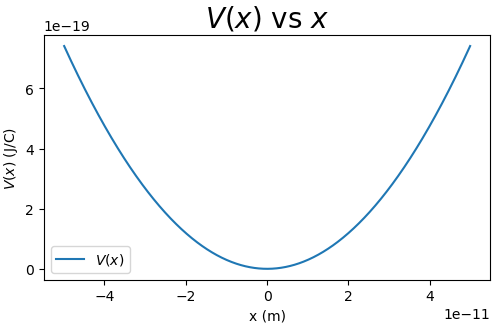
\includegraphics[width=7cm]{qho_potential.png} 
    \caption{Harmonic Oscillator Potential}
    \label{qho_potential}
\end{wrapfigure}

The potential of the quantum harmonic oscillator described by Table (\ref{system_parameters_for_qho}) over the discrete position grid $x_i$ is shown in in Fig. (\ref{qho_potential}).  It is a parabola centered on $x=0$.



\subsubsection{Numerical and Analytical Eigenergies}

The 1\textsuperscript{st} twenty (20) numerical eigenergies of the quantum harmonic oscillator system described by Table (\ref{system_parameters_for_qho}) are shown on Fig. (\ref{qho_eigenenergies}). As a check, the 1\textsuperscript{st} twenty (20) analytical eigenergies are shown on the same figure. The numerical eigenenergies show strong agreement with their analytical counterparts.

\vspace{3mm}
The eigenenergies plotted on Fig. (\ref{qho_eigenenergies}) are numerically listed in Table (\ref{qho_relative_errors}) along with their corresponding relative errors. Relative error is observed to increase with increasing $n$.
\vspace{1mm}
\begin{figure}[h]
    \centering
    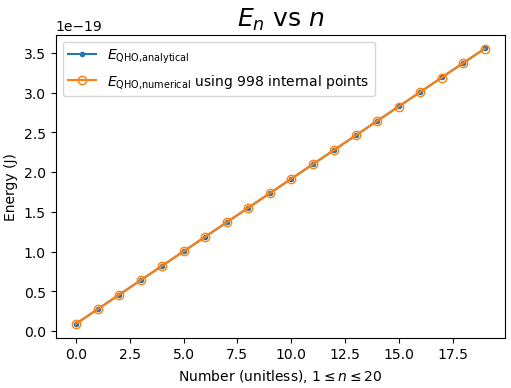
\includegraphics[width=9cm]{qho_eigenenergies.png}
    \caption{Numerical and Analytical Eigenenergies vs. $n$}
    \label{qho_eigenenergies}
\end{figure}
\begin{table}[h]
\begin{center}
    \footnotesize
    \begin{tabular}{|c|c|c|}
        \hline
        \textbf{System Parameter} & \textbf{Value} & \textbf{Notes} \\ \hline
        Start of Well & 5$\times 10^{-11}$ m & - \\ \hline
        End of Well & -5$\times 10^{-11}$ m & - \\ \hline 
        Total No. of Grid Points & 1000 & - \\ \hline 
        Mass of Trapped Particle &  1.99$\times 10^{-26}$ kg & Mass of One (1) Carbon Atom  \\ \hline 
        Oscillator Frequency & 1.728$\times 10^{12}$ s$^{-1}$ &  Einstein Frequency of Diamond, from Simon \cite[page 13]{Simon2013} \\ \hline
    \end{tabular}
\end{center}
\caption{System Parameters for Figs. (\ref{qho_potential},\ref{qho_eigenenergies})}
\label{system_parameters_for_qho}
\end{table}

\begin{table}[h]
\begin{center}
    \begin{tabular}{|c|c|c|c|c|}
        \hline
        $n$ & $E_n^\text{num}$ (eV) & $E_n^\text{exact}$ (eV) & $\Delta E_n\times 10^{6}$ (eV) & $\epsilon_{E,n}\times 10^{6}$ \\ \hline
    	0	&	0.057	&	0.057	&	-1.2	&	20.4	\\ \hline
		1	&	0.171	&	0.171	&	-5.8	&	34.1	\\ \hline
		2	&	0.284	&	0.284	&	-15.1	&	53.2	\\ \hline
		3	&	0.398	&	0.398	&	-29.1	&	73.0	\\ \hline
		4	&	0.512	&	0.512	&	-47.7	&	93.2	\\ \hline
		5	&	0.626	&	0.626	&	-71.0	&	113.4	\\ \hline
		6	&	0.740	&	0.740	&	-98.9	&	133.7	\\ \hline
		7	&	0.853	&	0.853	&	-131.5	&	154.1	\\ \hline
		8	&	0.967	&	0.967	&	-168.7	&	174.4	\\ \hline
		9	&	1.081	&	1.081	&	-210.6	&	194.8	\\ \hline
		10	&	1.195	&	1.195	&	-257.2	&	215.2	\\ \hline
		11	&	1.308	&	1.309	&	-308.4	&	235.6	\\ \hline
		12	&	1.422	&	1.422	&	-364.2	&	256.1	\\ \hline
		13	&	1.536	&	1.536	&	-424.8	&	276.5	\\ \hline
		14	&	1.650	&	1.650	&	-489.9	&	296.9	\\ \hline
		15	&	1.763	&	1.764	&	-559.8	&	317.4	\\ \hline
		16	&	1.877	&	1.878	&	-634.3	&	337.8	\\ \hline
		17	&	1.991	&	1.991	&	-713.4	&	358.2	\\ \hline
		18	&	2.104	&	2.105	&	-797.2	&	378.7	\\ \hline
		19	&	2.218	&	2.219	&	-885.7	&	399.1	\\ \hline
    \end{tabular}
\end{center}
\caption{Relative Errors for Fig. (\ref{qho_eigenenergies}) Eigenenergies}
\label{qho_relative_errors}
\end{table}

\newpage

\subsubsection{1\textsuperscript{st} Three Numerical Probability Densities}

The 1\textsuperscript{st} three (3) normalized probability densities, namely $P_n(x)$ where $n=0,1,2$, of the quantum harmonic oscillator may be seen in Fig. (\ref{first_three_probability_densities}). The general shape of these probability densities is as expected: $P_0(x)$ has no nodes, $P_1(x)$ has one node, and $P_2(x)$ has two nodes. Furthermore, it is also expected that probability peaks closer to the center $x=0$ are shorter than those farther away from the center; this pattern starts to be observed in $P_2(x)$, where the central probability peak is lower than the left and right probability peaks.

\begin{figure}[h]
    \centering
    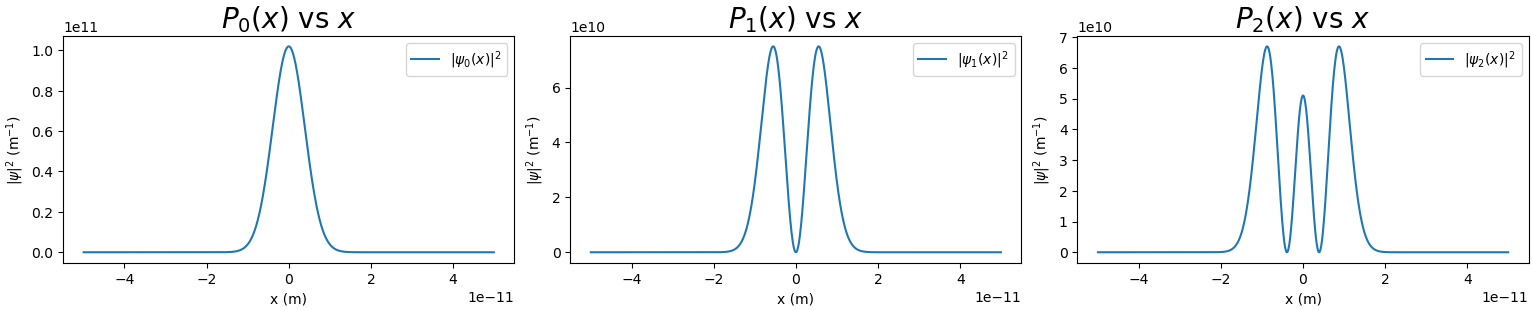
\includegraphics[width=16cm]{first_three_probability_densities.png} 
    \caption{Probability Distributions for $n=0,1,2$}
    \label{first_three_probability_densities}
\end{figure}

\newpage
\subsubsection{1\textsuperscript{st} Three Wavefunctions}

The 1\textsuperscript{st} three (3) normalized numerical wavefunctions and the 1\textsuperscript{st} three (3) normalized analytical wavefunctions, namely $P_n(x)$ where $n=0,1,2$, of the quantum harmonic oscillator may be seen in Fig. (\ref{first_three_wavefunctions}).

\begin{figure}[h]
    \centering
    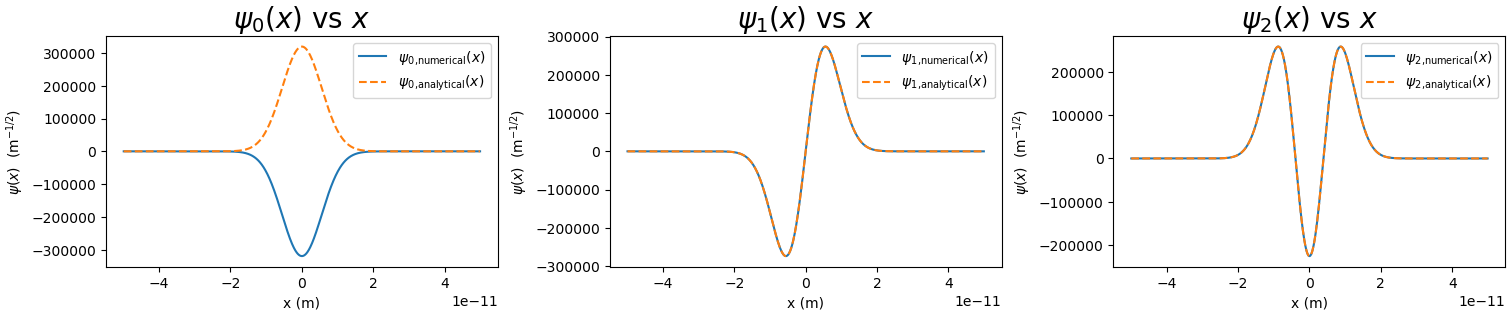
\includegraphics[width=16cm]{first_three_wavefunctions.png} 
    \caption{Wavefunctions for $n=0,1,2$}
    \label{first_three_wavefunctions}
\end{figure}

\subsubsection{$n=10$ Probability Density}

Thought this probability density function looked cool.
\begin{figure}[h]
    \centering
    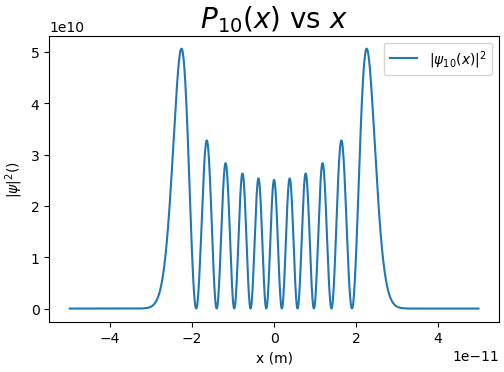
\includegraphics[width=10cm]{psi_10.png} 
    \caption{Wavefunction for $n=10$}
    \label{psi_10}
\end{figure}

\newpage
\subsubsection{Sensitivity to No. of Grid Points}
%
The relative errors for eigenenergies $n=0,1,2,3,4$ as a function of no. of grid points are shown in Table (\ref{grid_point_sensitivity_of_relative_error}). Relative error is observed to decrease with increasing no. of grid points.
\begin{table}[h]
\begin{center}
\begin{tabular}{|c|c|c|c|c|c|}
    \hline
    No. of Grid Points	&	$\epsilon_{E,0}\times 10^{3}$	&	$\epsilon_{E,1}\times 10^{3}$	&	$\epsilon_{E,2}\times 10^{3}$	&	$\epsilon_{E,3}\times 10^{3}$	&	$\epsilon_{E,4}\times 10^{3}$ \\ \hline
	30	&	24.90	&	42.47	&	68.15	&	97.05	&	128.21 \\ \hline
	50	&	8.57	&	14.39	&	22.64	&	31.38	&	40.41 \\ \hline
	100	&	2.09	&	3.48	&	5.44	&	7.49	&	9.58 \\ \hline
	500	&	0.08	&	0.14	&	0.21	&	0.29	&	0.37 \\ \hline
	1000	&	0.02	&	0.03	&	0.05	&	0.07	&	0.09 \\ \hline
\end{tabular}
\end{center}
\caption{Grid Point Sensitivity of Relative Error. Other system parameters (Table \ref{system_parameters_for_qho}) remain fixed.}
\label{grid_point_sensitivity_of_relative_error}
\end{table}

\subsubsection{Sensitivity to Grid Size}
%
The relative errors for eigenenergies $n=0,1,2,3,4$ as a function of grid size are shown in Table (\ref{grid_size_sensitivity_of_relative_error}). Relative error is generally observed to increase with increasing deviation from the original half-width $\ell$, with the increase being more drastic for decreasing half-widths.
\begin{table}[h]
\begin{center}
\begin{tabular}{|c|c|c|c|c|c|}
    \hline
    Well Half-Width	&	$\epsilon_{E,0}\times 10^{3}$	&	$\epsilon_{E,1}\times 10^{3}$	&	$\epsilon_{E,2}\times 10^{3}$	&	$\epsilon_{E,3}\times 10^{3}$	&	$\epsilon_{E,4}\times 10^{3}$ \\ \hline
	(1/8)$\ell$	&	1098.92	&	1698.93	&	2561.73	&	3480.53	&	4420.08 \\ \hline
	(1/5)$\ell$ &	145.38	&	302.67	&	564.11	&	878.31	&	1218.14 \\ \hline
	$\ell = 5\times 10^{-11}$ &	0.02	&	0.03	&	0.05	&	0.07	&	0.09 \\ \hline
	5$\ell$	&	0.51	&	0.85	&	1.33	&	1.83	&	2.33 \\ \hline
	8$\ell$	&	1.31	&	2.19	&	3.41	&	4.70	&	6.00 \\ \hline
\end{tabular}
\end{center}
\caption{Grid Size Sensitivity of Relative Error. Other system parameters (Table \ref{system_parameters_for_qho}) remain fixed.}
\label{grid_size_sensitivity_of_relative_error}
\end{table}

\newpage
\subsubsection{Average Energy and Heat Capacity}
%
The numerical average energy and numerical Einstein heat capacity of one (1) quantum harmonic oscillator are shown as functions of temperature in Fig. (\ref{average_energy_and_heat_capacity_of_one_oscillator}).
\begin{figure}[h]
    \centering
    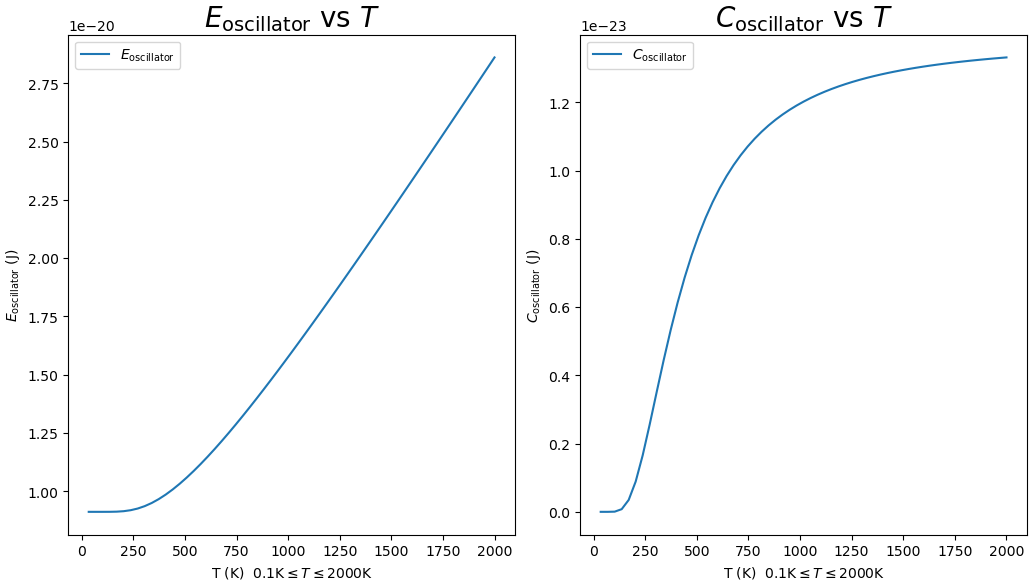
\includegraphics[width=16cm]{average_energy_and_heat_capacity_of_one_oscillator.png} 
    \caption{\small \centering Mean Internal Energy (left) and Heat Capacity (right) vs Temperature for One (1) Quantum Harmonic Oscillator}
    \label{average_energy_and_heat_capacity_of_one_oscillator}
\end{figure}





\subsection{Discussion}

The connection between Dirac notation and the position space Schrödinger equation, or equivalently the connection between the finite-grid and continuous interval problems, is elaborated upon in the subsection ``\textit{Numerical Methodology}.''

\vspace{3mm}
The numerical eigenergies were checked against the analytical eigenenergies by calculating their relative errors $\epsilon_{E,n}$ using the formula given in ``\textit{Eigenenergy Error Calculations}.''

\vspace{3mm}
The quantum harmonic oscillator modeled in this section is more accurately a quantum harmonic oscillator placed inside an infinite potential well with Dirichlet boundary conditions $\psi=0$. This means that the problem being solved is a fundamentally different problem and that the numerical eigenergies cannot come arbitrarily close to the analytical eigenergies.

\vspace{3mm}
Decreasing the grid spacing $\Delta x$ decreases the accuracy of the numerical eigenenergies since this decreases the total number of eigenergies that can be obtained from diagonalizing the Hamiltonian. Increasing or decreasing the well half-width $\ell$ also decreases the accuracy of the numerical eigenenergies since increasing it decreases the number of grid points located within the turning points of the classical counterpart of the quantum harmonic oscillator, while decreasing it puts the walls of the infinite potential well close to or within the classical turning points, respectively. High energy states are more susceptible to changes in $\ell$ than low energy states because the classical turning points of the former are farther away from the center $x=0$ and the corresponding wavefunctions occupy more space inside the infinite potential well.

\vspace{3mm}
The energy level weighting method and Bose-Einstein occupation term are equivalent since the independent oscillators are bosons with respect to each other, i.e. any two oscillators in the system can be in the same state and have the same energy at any time. However, the energy level weighting method can give average energies arbitrarily close to those calculated using the Bose-Einstein occupation term only if the former can accomodate infinitely many and infinitely large eigenenergies.

\vspace{3mm}
In this section, eigenenergies are displayed in terms of state number $n$ and not in terms of wavevector $k$ as they are for some other systems such as the free particle. This is because the average momentum, and therefore the average wavevector, of particles in infinite potential wells and/or quadratic potentials is 0, regardless of the energy of the particle.